\chapter{Grundlæggende begreber i talteori}
\label{chap:ch12}
Tal er fundamentet for matematikken. De repræsenterer mængder, målinger og sammenhænge i både abstrakt og konkret form. Studiet af tal går tusinder af år tilbage, og tidlige civilisationer som babylonierne, egypterne og grækerne lagde grunden til den moderne talteori. Disse oldtidskulturer udviklede den grundlæggende aritmetik, herunder addition, subtraktion, multiplikation og division, som der stadig undervises i i dag.

Talteori, som ofte kaldes »matematikkens dronning«, er en gren af matematikken, der beskæftiger sig med de hele tal og sammenhængene mellem dem. Den omfatter en lang række emner, herunder primtal, delelighed, modulær aritmetik og talsystemers egenskaber. Talteorien har en rig historie med betydelige bidrag fra matematikere som Euklid, der omkring 300 f.v.t. beviste, at der findes uendeligt mange primtal, og Pierre de Fermat, der er kendt for Fermats sidste sætning -- et problem, som matematikere sled med i over 350 år, indtil det endelig blev løst af Andrew Wiles i 1994.

\begin{figure}[h!]
    \centering
    % Shared diagram of the principal number sets.
% The part of R outside Q is exactly R \setminus Q; it is not a separate oval.
\begin{tikzpicture}[scale=0.7]
    % Complex numbers (outer set)
    \draw[thick, fill=mseComplex!35] (-12,-6) rectangle (10,5);
    \node at (8,4) {\Huge $\mathbb{C}$};

    % Real numbers. The area not covered by Q is the irrational numbers.
    \draw[thick, fill=mseReals] (-4,0) ellipse (7.8cm and 4.5cm);
    \node at (-3,3.8) {\Large $\mathbb{R}$};

    % Rational numbers and their nested subsets
    \draw[thick, fill=mseRationals] (-7,0) ellipse (4.5cm and 3cm);
    \node at (-11,0) {\Large $\mathbb{Q}$};

    \draw[thick, fill=mseIntegers] (-7,0) ellipse (3cm and 2cm);
    \node at (-9.5,0) {\Large $\mathbb{Z}$};

    \draw[thick, fill=mseNaturals] (-7,0) ellipse (2cm and 1.2cm);
    \node at (-7,0) {\Large $\mathbb{N}$};

    % These labels identify the two complementary regions.
    \node[align=center] at (0.7,0)
        {\Large $\mathbb{R}\setminus\mathbb{Q}$\\[-1pt]
         \small Irrationale tal};
    \node[align=center] at (7,0)
        {\Large $\mathbb{C}\setminus\mathbb{R}$\\[-1pt]
         \small Ikke-reelle komplekse tal};
\end{tikzpicture}

    \caption{Venn-diagram over tal}
    \label{fig:venn_num2}
\end{figure}

Gennem historien har talteorien udviklet sig fra en rent teoretisk disciplin til et felt med praktiske anvendelser i moderne teknologi. Kryptografi, videnskaben om sikker kommunikation, bygger for eksempel i høj grad på talteori, især på primtals egenskaber og modulær aritmetik. De algoritmer, der beskytter vores onlinetransaktioner og digitale kommunikation, er bygget på talteoriens principper.

I dette kapitel udforsker vi forskellige aspekter af tal og talteori. Vi begynder med det grundlæggende om hele tal, primtal og talsystemer og bevæger os gradvist videre til mere komplekse emner. Ved at forstå tallenes grundlæggende egenskaber får vi indsigt i de matematiske strukturer, som den digitale verden og meget mere hviler på.

\begin{remark}
Mange tal indgår i mere end én mængde. Tabel \ref{tab:number_types} giver et overblik over navne, egenskaber og symboler for de vigtigste taltyper.
\end{remark}

\begin{table}[ht]
\centering
\caption{Taltyper og deres egenskaber}
\label{tab:number_types}
\renewcommand{\arraystretch}{1.6} % Adjust the row height for the entire table
\small
\begin{tabularx}{\textwidth}{|>{\raggedright\arraybackslash}p{2.35cm}|>{\centering\arraybackslash}p{1.3cm}|>{\raggedright\arraybackslash}X|>{\raggedright\arraybackslash}X|}
\hline
Naturlige tal & \(\mathbb{N}\) & De ikke-negative hele tal (den konvention, der bruges i denne bog). & \(0, 1, 2, \ldots\) \\ \hline
Hele tal & \(\mathbb{Z}\) & Alle positive og negative hele tal. & \(\{\ldots, -2, -1, 0, 1, 2, \ldots\}\) \\ \hline
Rationale tal & \(\mathbb{Q}\) & Alle reelle tal, der kan skrives som en brøk, \(\frac{p}{q}\), hvor \(p\) og \(q\) er hele tal, og \(q \neq 0\). Alle hele tal er rationale tal, da \(1\) er et helt tal forskelligt fra nul. & \(\dfrac{1}{5}, \dfrac{5}{1} (=5), \dfrac{2}{3}, \dfrac{3}{2}, \dfrac{0}{3} (=0)\) \\ \hline
Irrationale tal & \(\mathbb{R}\ \setminus \mathbb{Q}\) & Alle reelle tal, der ikke kan skrives som en brøk, hvis tæller og nævner er hele tal. & \(\pi, \sqrt{2}, \sqrt{3}\) \\ \hline
Reelle tal & \(\mathbb{R}\) & Omfatter alle tal på tallinjen. & \(\dfrac{1}{5}, \sqrt{\dfrac{1}{5}}, 0, -2\) \\ \hline
\makecell[l]{Rene imaginære\\tal} & \(i\mathbb{R}\) & Tal på formen \(bi\), hvor \(b\) er reel, og \(i^2=-1\). & \(\begin{array}{l}
\vspace{3pt} 3i = \sqrt{-9},\ -5i = -\sqrt{-25}, \\
3\sqrt{2}i = \sqrt{-18} \vspace{3pt}
\end{array}\) \\ \hline
Komplekse tal & \(\mathbb{C}\) & Alle tal på formen $a+bi$, hvor $a,b\in\mathbb{R}$, og $i^2=-1$. & $1+2 i, 1, i,-3 i, 0,-5+i$ \\ \hline
\end{tabularx}
\end{table}

\begin{remark}
    I Figur \ref{fig:venn_num2} udgør de rationale og de irrationale tal en partition af de reelle tal. Ethvert komplekst tal har formen $a+bi$ med $a,b\in\mathbb{R}$. De reelle tal er netop dem med $b=0$; komplekse tal med $b\neq0$ er ikke-reelle. Rene imaginære tal har $a=0$ og udgør kun én delmængde af de komplekse tal, ikke alle ikke-reelle komplekse tal.
\end{remark}

\section{Taltyper}
Lad os nu fokusere på de delmængder af de reelle tal, der står i tabellen: naturlige tal, ikke-negative hele tal (på engelsk \emph{whole numbers}), hele tal, rationale tal, irrationale tal og reelle tal. Overblikket ovenfor placerer disse mængder i det større system af komplekse tal.

\subsection*{Naturlige tal}
Vi begynder med de naturlige tal. Vi skelner mellem de ikke-negative hele tal: $0, 1, 2, 3, \ldots$ og tælletallene (på engelsk \emph{counting numbers}): $1, 2, 3, \ldots$. Disse tal bruges primært til at tælle med. Naturlige tal opfattes ofte som eksakte værdier (fx har en bil 4 dæk, og en edderkop har 8 ben). I nogle sammenhænge kan de dog bruges som tilnærmelser (fx var der cirka 1000 mennesker i mængden).

En af de naturlige tals centrale egenskaber er, at de er \textit{lukkede} under visse operationer, såsom addition og multiplikation. Det betyder, at hvis du tager to vilkårlige naturlige tal og lægger dem sammen eller ganger dem, vil resultatet altid være et naturligt tal. Hvis $a$ og $b$ for eksempel er naturlige tal, er både $a + b$ og $a \times b$ også naturlige tal.

Der er meget lidt enighed om, hvorvidt symbolet $\mathbb{N}$ omfatter 0. Derfor betegnes mængden af ikke-negative hele tal (som omfatter 0) ofte $\mathbb{W}$ (af engelsk »whole numbers«).

\subsection*{Hele tal}
De hele tal er talteoriens grundlæggende byggesten. De består af de ikke-negative hele tal og deres negative modstykker. Formelt omfatter de hele tal tal som $\ldots,-3,-2,-1,0,1,2,3, \ldots$ Grundlæggende regneoperationer som addition og multiplikation følger bestemte regler:

\begin{custombox}{{Kommutative, associative og distributive love}}


    \begin{itemize}
    \item Kommutativitet: $a+b=b+a$
    \item Associativitet: $(a+b)+c=a+(b+c)$
    \item Den distributive lov: $a \times(b+c)=a \times b+a \times c$
    \end{itemize}
    
\end{custombox}

De hele tal er en grundlæggende talmængde i matematikken og betegnes med symbolet $\mathbb{Z}$. Mængden omfatter alle positive og negative hele tal samt nul. De hele tal udvider de naturlige tal ved at inddrage deres additive inverse, så subtraktion fuldt ud kan udføres inden for mængden.

\textbf{Additivt neutralt element:} Tallet \(0\) kaldes det additive neutrale element. Det skyldes, at det for ethvert helt tal \(a\) gælder, at værdien af \(a\) ikke ændres, når man lægger nul til. Matematisk udtrykkes denne egenskab som \(0 + a = a + 0 = a\). Det neutrale element er afgørende, fordi det sikrer, at mængden af hele tal forbliver stabil under addition.
    
 \textbf{Multiplikativt neutralt element:} Tilsvarende fungerer tallet \(1\) som det multiplikative neutrale element. For ethvert helt tal \(a\) gælder, at multiplikation med én lader værdien af \(a\) være uændret: \(1 \times a = a \times 1 = a\). Denne egenskab ligger til grund for de hele tals stabilitet under multiplikation og bevarer mængdens integritet.
    
\textbf{Additiv invers:} Til ethvert helt tal \(a\) findes en tilhørende additiv invers, som betegnes \(-a\). Den additive inverse er defineret sådan, at når \(a\) og \(-a\) lægges sammen, er resultatet det additive neutrale element, nul: \(a + (-a) = 0\). Denne egenskab gør det muligt at udføre subtraktion inden for mængden af hele tal, da subtraktion kan opfattes som addition af en additiv invers.

\begin{custombox}{Lukkethed}
    \textbf{Addition:} Mængden af hele tal er lukket under addition. Det betyder, at hvis du tager to vilkårlige hele tal og lægger dem sammen, vil summen altid være et helt tal. Hvis \(a\) og \(b\) for eksempel er hele tal, er \(a + b\) også et helt tal. Denne lukkethed sikrer, at mængden af hele tal er stabil og fuldstændig under addition. Uanset hvor mange gange du lægger hele tal sammen, vil resultatet altså forblive inden for mængden af hele tal.

\textbf{Multiplikation:} Mængden af hele tal er også lukket under multiplikation. Hvis du ganger to vilkårlige hele tal, vil produktet altid være et helt tal. Hvis \(a\) og \(b\) for eksempel er hele tal, er \(a \times b\) også et helt tal. Denne egenskab garanterer, at multiplikation ligesom addition ikke giver resultater uden for mængden af hele tal, og bevarer derved mængdens integritet under multiplikation.

\end{custombox}

Der er universel enighed om, at definitionen af et helt tal er klar og præcis. Når du er i tvivl, er det derfor tilrådeligt at omtale tal i denne mængde som »hele tal«. Når du specifikt kun vil omtale de positive hele tal, er det både præcist og professionelt eksplicit at skrive »positive hele tal«. Denne terminologi sikrer ikke blot klarhed, men viser også en sikker forståelse af matematiske konventioner. 

Husk, at nul hverken er positivt eller negativt. Når man taler om delmængder af de hele tal, skal man derfor tage nøje hensyn til dette:

\begin{itemize}
    \item \textbf{Hele tal:} $\mathbb{Z} = \{\ldots,-4,-3,-2,-1,0,1,2,3,4, \ldots\}$
    \item \textbf{Negative hele tal:} $\mathbb{Z}^- = \{\ldots,-4,-3,-2,-1\}$
    \item \textbf{Positive hele tal:} $\mathbb{Z}^+ = \{1,2,3,4, \ldots\}$
    \item \textbf{Ikke-negative hele tal:} $\mathbb{Z}_0^+ = \mathbb{Z}_{\geq 0} = \{0,1,2,3,4, \ldots\}$
    \item \textbf{Ikke-positive hele tal:} $\mathbb{Z}_0^- = \mathbb{Z}_{\leq 0} = \{\ldots,-4,-3,-2,-1, 0\}$
\end{itemize}

Denne notation bør være i overensstemmelse med gængse matematiske konventioner.

\subsection*{Rationale tal}
Rationale tal, som betegnes med symbolet $\mathbb{Q}$, er tal, der kan skrives som kvotienten af to hele tal, hvor tælleren er et vilkårligt helt tal, og nævneren er et helt tal forskelligt fra nul. Formelt kan et rationalt tal skrives som $\frac{a}{b}$, hvor $a \in \mathbb{Z}$ og $b \in \mathbb{Z} \setminus \{0\}$. Denne talmængde er grundlæggende i matematikken, da den giver mulighed for at repræsentere brøker og forhold og dermed for en lang række regneoperationer. De rationale tal er således en generalisering af de almindelige brøker, som vi så i \autoref{chap:ch0}. De kan repræsentere ethvert tal, der kan skrives som et endeligt eller periodisk decimaltal.

En af de rationale tals centrale egenskaber er, at ethvert rationalt tal forskelligt fra nul har en \textit{multiplikativ invers}. Den multiplikative inverse til et rationalt tal $\frac{a}{b}$ er det rationale tal $\frac{b}{a}$, forudsat at $a \neq 0$. Betydningen af den multiplikative inverse ligger i, at når et tal ganges med sin inverse, er resultatet det \textit{multiplikative neutrale element}, som er 1. For ethvert rationalt tal $\frac{a}{b}$ betegnes den inverse med andre ord $\left(\frac{a}{b}\right)^{-1} = \frac{b}{a}$, og vi har:

\[
\frac{a}{b} \times \frac{b}{a} = \frac{ab}{ba} = 1
\]

Denne egenskab sikrer, at de rationale tal er lukkede under multiplikation og division (bortset fra division med nul), hvilket gør dem til en robust og alsidig talmængde til forskellige matematiske operationer.

De rationale tal ligger tæt på tallinjen. Det betyder, at der mellem to vilkårlige rationale tal findes et andet rationalt tal. Denne egenskab gør mængden af rationale tal særligt vigtig i studiet af de reelle tal, da den gør det muligt at tilnærme irrationale tal med en vilkårlig ønsket nøjagtighed.

\subsection*{Irrationale tal}
Irrationale tal, som betegnes med symbolet $\mathbb{R} \setminus \mathbb{Q}$, er reelle tal, der ikke kan skrives som kvotienten af to hele tal. I modsætning til rationale tal, som har en periodisk eller endelig decimalfremstilling, er decimalfremstillingen af et irrationalt tal hverken periodisk eller endelig. Denne egenskab gør irrationale tal fundamentalt forskellige fra rationale tal, da de ikke kan repræsenteres præcist som brøker.

Nogle af de mest kendte eksempler på irrationale tal er:

\begin{itemize}
    \item \textbf{Pi} ($\pi$): $\pi$ er måske det mest kendte irrationale tal og er forholdet mellem en cirkels omkreds og dens diameter. Værdien er cirka $3.14159\ldots$, men decimalfremstillingen fortsætter uendeligt uden at gentage sig. $\pi$ spiller en afgørende rolle i geometri, trigonometri og infinitesimalregning.

    \item \textbf{Det gyldne snit} ($\phi$): Det gyldne snit, $\phi \approx 1.61803\ldots$, er et irrationalt tal, der ofte optræder i naturen, kunsten og arkitekturen. Det er defineret som den positive løsning til ligningen $x^2 - x - 1 = 0$, og det er grænseværdien for forholdet mellem på hinanden følgende Fibonaccital.

    \item \textbf{Kvadratroden af 2} ($\sqrt{2}$): Kvadratroden af 2, cirka $1.41421\ldots$, er længden af diagonalen i et kvadrat med sidelængden 1. Tallet har historisk betydning, fordi oldtidens grækere, især pythagoræerne, med opdagelsen af det afslørede, at der findes tal, som ikke kan skrives som forholdet mellem to hele tal. Pythagoras' sætning siger, at i en retvinklet trekant er kvadratet på hypotenusen lig med summen af kvadraterne på de to andre sider. For en retvinklet trekant, hvor begge kateter har længden 1, er hypotenusen $\sqrt{2}$, hvilket viser, at $\sqrt{2}$ ikke kan være et rationalt tal.

    \item \textbf{Eulers tal} ($e$): Tallet $e \approx 2.71828\ldots$ er grundtallet for den naturlige logaritme og en grundlæggende konstant i matematikken, især i infinitesimalregning og kompleks analyse. Tallet $e$ opstår naturligt i forskellige vækstprocesser, såsom renters rente og befolkningsvækst.
\end{itemize}

Irrationale tal udfylder hullerne mellem de rationale tal på tallinjen og gør dermed de reelle tal til en kontinuert mængde. Ligesom de rationale tal har de dog også vigtige egenskaber. Selv om irrationale tal for eksempel ikke har en simpel brøkfremstilling, er de alligevel uundværlige til at repræsentere de længder, arealer og rumfang, som ikke kan beskrives med rationale tal alene.

\subsection*{Reelle tal}
Reelle tal, som betegnes med symbolet $\mathbb{R}$, danner grundlaget for det meste af den matematiske analyse og er uundværlige til at beskrive kontinuerte størrelser. Mængden af reelle tal består af både de rationale tal ($\mathbb{Q}$) og de irrationale tal ($\mathbb{R} \setminus \mathbb{Q}$) og omfatter dermed alle tal, der kan placeres på tallinjen. Selv om både rationale og irrationale tal er en del af det reelle talsystem, adskiller deres egenskaber sig markant:

\begin{custombox}{Ligheder og forskelle mellem rationale og irrationale tal}
    \begin{itemize}
    \item \textbf{Repræsentation:} Rationale tal kan repræsenteres som brøker, mens irrationale tal ikke kan. Denne forskel gør irrationale tal mere komplicerede at håndtere, især i regneoperationer.

    \item \textbf{Decimalfremstilling:} Decimalfremstillingen af rationale tal er enten endelig eller periodisk, mens decimalfremstillingen af irrationale tal er uendelig og ikke-periodisk.

    \item \textbf{Lukkethed:} De rationale tal er lukkede under addition, subtraktion, multiplikation og division (bortset fra division med nul). De irrationale tal er ikke lukkede under disse operationer; for eksempel kan summen eller produktet af to irrationale tal undertiden være rationalt.

    \item \textbf{Tæthed:} De rationale tal ligger tæt på den reelle tallinje. Det betyder, at der mellem to vilkårlige rationale tal findes et andet rationalt tal. De irrationale tal ligger også tæt, men på en komplementær måde: De udfylder de »huller«, som de rationale tal efterlader, og sikrer, at den reelle tallinje er kontinuert uden afbrydelser.
\end{itemize}
\end{custombox}

Den reelle tallinje er en kontinuert, ubrudt linje, der strækker sig uendeligt i begge retninger. Hvert punkt på linjen svarer til ét bestemt reelt tal, uanset om det er rationalt eller irrationalt. Det er denne kontinuitet, der gør det muligt at bruge de reelle tal til at modellere kontinuerte fænomener i naturen, såsom tid, afstand og temperatur.

\section{Egenskaber ved hele tal og modulær aritmetik}
I kapitel \ref{chap:ch0} introducerede vi begrebet faktor. En faktor er en del af en størrelse, som regel et helt tal eller et polynomium, der ganget med andre faktorer giver hele størrelsen.

I talteori er en faktor i et tal \(n\) det samme som en \textbf{divisor} i \(n\). Mere præcist er en divisor i et helt tal \(n\) et helt tal \(d\), der går op i \(n\), så resultatet bliver et andet helt tal.

En positiv \textbf{ægte divisor} er en positiv divisor i et tal \(n\), bortset fra \(n\) selv. Tilsvarende er en \textbf{ægte faktor} i et positivt helt tal \(n\) en faktor i \(n\), der er forskellig fra 1 og \(n\).

Faktorerne i 12 er for eksempel:

\[
1, 2, 3, 4, 6, 12
\]

I denne liste er 2, 3, 4 og 6 ægte faktorer i 12. Det betyder, at de er mindre end 12 selv, men større end 1.

Et primtal er et naturligt tal større end 1, som ikke har andre positive divisorer end 1 og sig selv. Et primtal kan med andre ord ikke dannes ved at gange to mindre naturlige tal. De første primtal er:

\[
2, 3, 5, 7, 11, 13, 17, 19, 23, 29, \ldots
\]

Bemærk, at 2 er det eneste lige primtal, fordi ethvert andet lige tal kan divideres med 2 og dermed er \textit{sammensat}. Et \textbf{sammensat tal} er i modsætning til et primtal et naturligt tal større end 1, som går op med mindst ét andet positivt helt tal end 1 og sig selv. For eksempel er 6 et sammensat tal, fordi det kan skrives som \(6 = 2 \times 3\).

\subsection*{Primfaktoropløsning}
Primfaktoropløsning er processen, hvor et sammensat tal opløses i et produkt af dets primfaktorer. For ethvert sammensat tal er denne opløsning entydig, bortset fra faktorernes rækkefølge. Se for eksempel på tallet 60:
\[
60 = 2 \times 2 \times 3 \times 5 = 2^2 \times 3 \times 5
\]
Her er 2, 3 og 5 primfaktorer i 60, og $2^2 \times 3 \times 5$ er den \textbf{kanoniske faktorisering} af 60 -- normalt kalder vi den blot primfaktoropløsningen.

\begin{theorem}{Aritmetikkens fundamentalsætning}
Ethvert helt tal større end 1 kan skrives entydigt som et produkt af primtal, bortset fra faktorernes rækkefølge.
\end{theorem}

Denne sætning understreger primtallenes betydning som »byggesten« for alle naturlige tal.

\begin{example}

\[
84 = 2^2 \times 3 \times 7
\]
\end{example}

Uanset hvordan du faktoriserer 84, ender du altid med de samme primtal (2, 3 og 7), selv om rækkefølgen kan variere.

Primfaktoropløsningen giver en entydig fremstilling af tallet ved hjælp af dets primfaktorer.

\subsection*{Største fælles divisor (GCD)}
Den største fælles divisor (GCD, af engelsk \emph{greatest common divisor}) af to eller flere hele tal, som også kaldes \textit{største fælles faktor} (på engelsk \textit{highest common factor}, HCF, eller \textit{greatest common factor}, GCF), er det største positive hele tal, der går op i hvert af de givne tal uden at efterlade en rest. For at bestemme GCD bruger man almindeligvis primfaktoropløsningen af de involverede tal. GCD findes derefter ved at gange de fælles primfaktorer med de mindste eksponenter fra tallenes primfaktoropløsninger.

Se for eksempel på, hvordan man finder GCD af 24 og 36:
\[
24 = 2^3 \times 3, \quad 36 = 2^2 \times 3^2
\]
De fælles primfaktorer er 2 og 3. Dermed er GCD:
\[
\text{GCD} = 2^2 \times 3 = 12
\]

\begin{example} Find GCD af 36 og 120

\begin{solution}
    

Pilene viser de tal, vi har valgt.

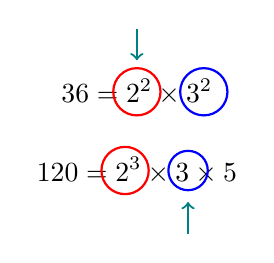
\begin{tikzpicture}
    % First line
    \node at (0, 0) {\(\displaystyle 36 = 2^2 \times 3^2\)};
    
    % Second line
    \node at (0, -1) {\(\displaystyle 120 = 2^3 \times 3 \times 5\)};
    
    % Circles around specific elements
    \draw[red, thick] (0, 0.0) circle(0.3); % Circle around 2^2
    \draw[blue, thick] (0.85, 0.0) circle(0.3); % Circle around 3^2
    
    \draw[red, thick] (-0.15, -1) circle(0.3); % Circle around 2^3
    \draw[blue, thick] (0.65, -1) circle(0.25); % Circle around 3

    % Arrows
    \draw[thick, teal, ->] (0, 0.8) -- (0, 0.4);
    \draw[thick, teal, ->] (0.65, -1.8) -- (0.65, -1.4);
\end{tikzpicture}

Vi ser, at 2 og 3 er fælles faktorer, og vælger dem med de mindste eksponenter:

\[
GCD = 2^2\times 3 = 12
\]
\end{solution}

\end{example}
 
\subsection*{Mindste fælles multiplum (LCM)}
Det mindste fælles multiplum (LCM, af engelsk \emph{least common multiple}) af to eller flere hele tal er det mindste positive hele tal, som hvert af de givne tal går op i. LCM kan også bestemmes ved hjælp af tallenes primfaktoropløsning. 

Se for eksempel på, hvordan man finder LCM af 24 og 36:
\[
24 = 2^3 \times 3, \quad 36 = 2^2 \times 3^2
\]
LCM fås ved at tage den højeste potens af hver primfaktor, der optræder i opløsningen af et af tallene:
\[
\text{LCM} = 2^3 \times 3^2 = 72
\]

\begin{example} Find LCM af 12 og 18.

\begin{solution}
\[
12 = 2^2\times 3
\]
\[
18 = 2 \times 3^2
\]

De højeste potenser, der optræder i en af opløsningerne, er $2^2$ og $3^2$, så

\[
LCM = 2^2 \times 3^2 = 36
\]
    
\end{solution}
    
\end{example}

\begin{example} Find LCM af 80 og 120

\begin{solution}
    

Pilene viser de tal, vi har valgt.

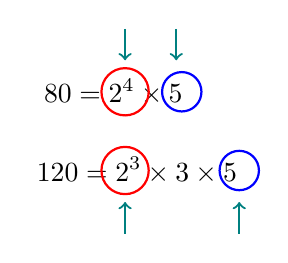
\begin{tikzpicture}
    % First line
    \node at (0, 0) {\(\displaystyle 80 = 2^4 \times 5\)};
    
    % Second line
    \node at (0.3, -1) {\(\displaystyle 120 = 2^3 \times 3 \times 5\)};
    
    % Circles around specific elements
    \draw[red, thick] (0.15, 0.0) circle(0.3); % Circle around 2^2
    \draw[blue, thick] (0.87, 0.0) circle(0.25); % Circle around 3^2
    
    \draw[red, thick] (0.15, -1) circle(0.3); % Circle around 2^3
    \draw[blue, thick] (1.6, -1) circle(0.25); % Circle around 3

    % Arrows
    \draw[thick, teal, ->] (0.15, 0.8) -- (0.15, 0.4);
    \draw[thick, teal, ->] (0.8, 0.8) -- (0.8, 0.4);
    \draw[thick, teal, ->] (0.15, -1.8) -- (0.15, -1.4);
    \draw[thick, teal, ->] (1.6, -1.8) -- (1.6, -1.4);
\end{tikzpicture}

Til LCM vælger vi den største eksponent for hvert primtal, der optræder i en af opløsningerne:

\[
LCM = 2^4\times 3 \times 5 = 240
\]
\end{solution}

\end{example}


\subsection*{Sammenhængen mellem GCD og LCM}

En vigtig sammenhæng mellem GCD og LCM af to tal \(a\) og \(b\) er givet ved formlen:
\[
\text{GCD}(a, b) \times \text{LCM}(a, b) = |a b|
\]
Med tallene 24 og 36 får vi for eksempel:
\[
12 \times 72 = 24 \times 36 = 864
\]
Denne sammenhæng er et stærkt værktøj til at løse problemer inden for delelighed, talteori og algebra.

Studiet af primtal og faktorer er grundlæggende i matematikken og giver vigtige værktøjer til at forstå tallenes struktur. Begreberne primfaktoropløsning, aritmetikkens fundamentalsætning og beregning af GCD og LCM er ikke kun afgørende i teoretisk matematik, men også i praktiske anvendelser som kryptografi, kodningsteori og analyse af algoritmer.

\subsection*{Divisorer og rester}
\label{sec:2.3Mod}
Division med hele tal kan være vanskelig, da resultatet ikke altid er et helt tal. Ofte giver en division en rest. For eksempel er

\[
9 = 2 \times 4 + 1.
\]

Her giver division af 9 med 4 en \textit{rest} på 1.

Generelt gælder det for hele tal \(a\neq0\) og \(b\), at der findes entydigt bestemte hele tal $q$ og $r$, så

\[
b = q a + r, \qquad 0\leq r<|a|.
\]

Det hele tal $q$ er kvotienten, og \(r\) er resten. Hvis \(r=0\), går \(a\) op i \(b\), hvilket skrives \(a \mid b\). For eksempel gælder \(2 \mid 128\) og \(7 \mid 49\), men \(3 \nmid 4\).

I denne bog bruges \emph{faktor} og \emph{divisor} i flæng. En positiv ægte divisor i et positivt helt tal $b$ er en positiv divisor, der er forskellig fra $b$ selv. Et primtal har derfor præcis to positive divisorer, 1 og sig selv, og ingen ægte divisor større end 1.

\subsection*{Modulær aritmetik}
Operatoren \texttt{mod}, som man ofte støder på i programmering, giver resten efter division. For eksempel:
\begin{enumerate}
    \item \(25 \bmod 4 = 1\), fordi \(25 \div 4 = 6\) med en rest på 1.
    \item \(19 \bmod 5 = 4\), da \(19 = 3 \times 5 + 4\).
    \item \(24 \bmod 5 = 4\).
    \item \(99 \bmod 11 = 0\).
\end{enumerate}

Selv om der i programmeringssprog er nogle konventionsafhængige detaljer for negative operander, fokuserer vi på positive hele tal. Kongruensnotation udtrykker, at to hele tal har samme rest: $24\equiv4\pmod 5$ og $21\equiv0\pmod 7$. Det er forskelligt fra restoperationen, som skrives $24\bmod5=4$ og $21\bmod7=0$.

Modulær aritmetik kaldes undertiden uraritmetik. Forestil dig et 24-timersur: 09:00 betyder klokken 9 om morgenen, mens 21:00 betyder klokken 9 om aftenen. Hvis en rejse starter kl. 07:00 og varer 25 timer, er ankomsttiden kl. 08:00 næste dag. Matematisk kan det udtrykkes som \(7 + 25 = 32\) og \(32 \bmod 24 = 8\). Vi starter altså ved 7 og bevæger os 25 timer frem på urskiven, så vi lander på 8.
